%
% $Id: matimet.tex,v 1.2 2002-03-13 10:14:20 jabril Exp $
%
%2345678901234567890123456789012345678901234567890123456789012345678901234567890
%        1         2         3         4         5         6         7         8
%
\chap{Material i M�todes}

\sctn{Predicci� Computacional de Gens}

\subsctn{{\gnid}}

\begin{figure}[!t]
\begin{center}
\begin{minipage}[t]{0.5\linewidth}
\fbox{
 \includegraphics[width=0.45\linewidth]{./psfigures/geneid_flowchart.ps}
} % fbox
\end{minipage}
\hspace{0.25cm}
\begin{minipage}[t]{0.45\linewidth}
\cpt{fig:geneidflowchart}
    {Diagrama de la estructura interna del {\gnid}.}
    {Estructura interna del programa de predicci� computacional de gens {\gnid}... }
\end{minipage}
\end{center}
\end{figure}



\sctn{Analitzant la homologia entre humans i ratolins}


\begin{figure}[!t]
\begin{center}
\begin{minipage}[t]{0.5\linewidth}
\fbox{
\begin{minipage}[c][5cm][c]{\linewidth}\hfill\end{minipage}
% \includegraphics[width=0.45\linewidth]{./psfigures/.ps}
} % fbox
\end{minipage}
\hspace{0.25cm}
\begin{minipage}[t]{0.45\linewidth}
\cpt{fig:humushomology}
    {Analitzant la homologia entre humans i ratolins.}
    {...}
\end{minipage}
\end{center}
\end{figure}


\subsctn{{\sgp}}


\sctn{Protocol de reanotaci� del genoma hum�}


\begin{figure}[!t]
\begin{center}
\begin{minipage}[t]{0.5\linewidth}
\fbox{
\begin{minipage}[c][5cm][c]{\linewidth}\hfill\end{minipage}
% \includegraphics[width=0.45\linewidth]{./psfigures/.ps}
} % fbox
\end{minipage}
\hspace{0.25cm}
\begin{minipage}[t]{0.45\linewidth}
\cpt{fig:humgenreannot}
    {Diagrama del proc�s de reanotaci� del genoma hum� basat en la homologia amb ratol�.}
    {...}
\end{minipage}
\end{center}
\end{figure}
